\documentclass{article}

%package setup
\usepackage{graphicx}
\usepackage{amsmath}
\usepackage{fancyhdr}
\usepackage[margin=1in]{geometry}
\usepackage{comment}
\usepackage{placeins}
\usepackage{parskip}
\usepackage{subcaption}
\usepackage{appendix}
\usepackage{soul}
\usepackage{comment}
\usepackage[hidelinks]{hyperref}
\usepackage{matlab-prettifier}
\usepackage{minted}
\usepackage{enumitem}
\usepackage{float}
\usepackage{textcomp, gensymb}
\usepackage{caption}


\pagestyle{fancy}
\fancyhf{} % Clear header/footer settings
\rhead{\thepage} % Page number on the right in the header
\lhead{ASE375 Lab Report 5} % Your lab report title on the left

\begin{document}

\begin{titlepage}
  \centering
  
\includegraphics[width=10cm]{ase-logo-formal.png}  % Adjust the width as needed
  \vspace{1cm}  % Add some vertical space
 
  \Large \textbf{ASE 375 Electromechanical Systems}\\
  \large \textbf{Section 14115}\\
  \vspace{0.5cm}
  \textbf{Monday: 3:00 - 6:00 pm}\\
 
  \vspace{1cm}
 
  \hrule
  \vspace{0.5cm}
 
  \Huge \textbf{Report 6:\\
  Measuring Dynamic Response with Accelerometers}\\
  \Huge \textbf{}\\
 
  \vspace{0.5cm}
  \hrule
 
  \vspace{1cm}
 
  \normalsize \textbf{Andrew Doty, Andres Suniaga, Dennis Hom}\\
  \normalsize \textbf{Due Date: 03/25/2024}
 
\end{titlepage}
\newpage

\tableofcontents
\thispagestyle{empty}
\newpage

\section{Introduction}
This experiment explores the dynamic response of a built-up wing from measurements using (1) a Piezoelectric accelerometer and (2) a Micro-Electro-Mechanical system (MEMS) accelerometer. The goal of this lab experiment is to learn how the accelerometers work by performing a resonance assessment profile (rap or impulse) test on the make-shift wing. 
\vspace{5mm}

The piezoelectric accelerometer cannot measure static quantities, meaning it does not take into the account the force exerted by gravity. On the other hand, the MEMS accelerometer does take into account the gravitational force in its measurements. This lab experiment provides a foundation for understanding the operational aspects of the accelerometers as well as a rap test use-case that show how these sensors are applied in testing of aircraft surfaces.

\section{Equipment}
Measurement devices and hardware used in this lab include:
\begin{itemize}

\item Built-Up Wing Model: 
\vspace{1mm}

In this lab we will use a scaled-down wing model for performing the rap test. This form of experiment is useful in application as rap tests are performed on control surfaces of aircraft.

\begin{figure}[H]
    \centering
    \caption{Sketch of Built-Up Wing Model setup}hi
    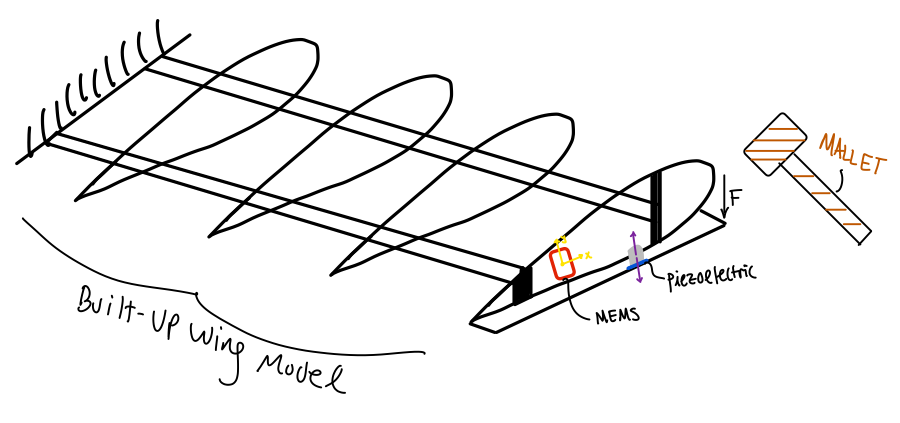
\includegraphics[width = 0.8\textwidth]{lab6images/wingmodellab6.png}
    \label{fig:wingmodel}
\end{figure}
\vspace{2.5mm}

\item Piezoelectric Accelerometer (IMI 660)
\vspace{1mm}

An IMI Series 660 accelerometer is used in the experiment. This Piezoelectric accelerometer only measures acceleration in one direction, and is placed on the built-up wing model as shown in Figure \ref{fig:wingmodel}.\\[1mm]
The operational principle of the Piezoelectric accelerometer is in it piezoelectric crystal, which generates charge from applied stress. It converts mechanical energy into electrical energy. The crystal acts like a capacitor (stores electrical energy). Operational Voltage = $5\text{V}$
\vspace{2.5mm}

\item MEMS Accelerometer (ADXL335)
\vspace{1mm}

The ADXL335 is a small 3-Axis MEMS Accelerometer which operates based on differential capacitance. An applied force or acceleration will change the capacitance within the MEMS accelerometer. In this experiment, the MEMS accelerometer is placed as shown in Figure \ref{fig:wingmodel}, using only the X-and Y-axes. Operational Voltage = $3.3\text{V}$
\vspace{2.5mm}

\item Brass Mallet: 
\vspace{1mm}

A brass mallet is used to apply a tap force to the built-up wing model as shown in Figure \ref{fig:wingmodel}. 
\vspace{2.5mm}

\item DAQ, NI-9215 Voltage Input Module, and LabVIEW:
\vspace{1mm}

Data Acquisition System used to process sample measurements into digital data. NI-9215 is an analog input module used to measure the output voltage signals of sensors and send it through the DAQ system. LabVIEW used to model these output voltages read from the DAQ of the accelerometer measurements. We connect to the $3.3 \text{V}$ and $5 \text{V}$ ports of the DAQ for our experiment.
\vspace{2.5mm}

\item Solderless Breadboard, Jumper Wires: 
\vspace{1mm}

Used to make connections to the input analog modules and to construct circuits. In this lab we connect the accelerometer inputs to the breadboard for power, ground, and signal to the measurement axes.

\end{itemize}

\section{Procedure}
Before beginning the experiment, we must build the block diagram which will be executed by LabVIEW to gather our accelerometer measurements. 

\begin{figure}[H]
    \centering
    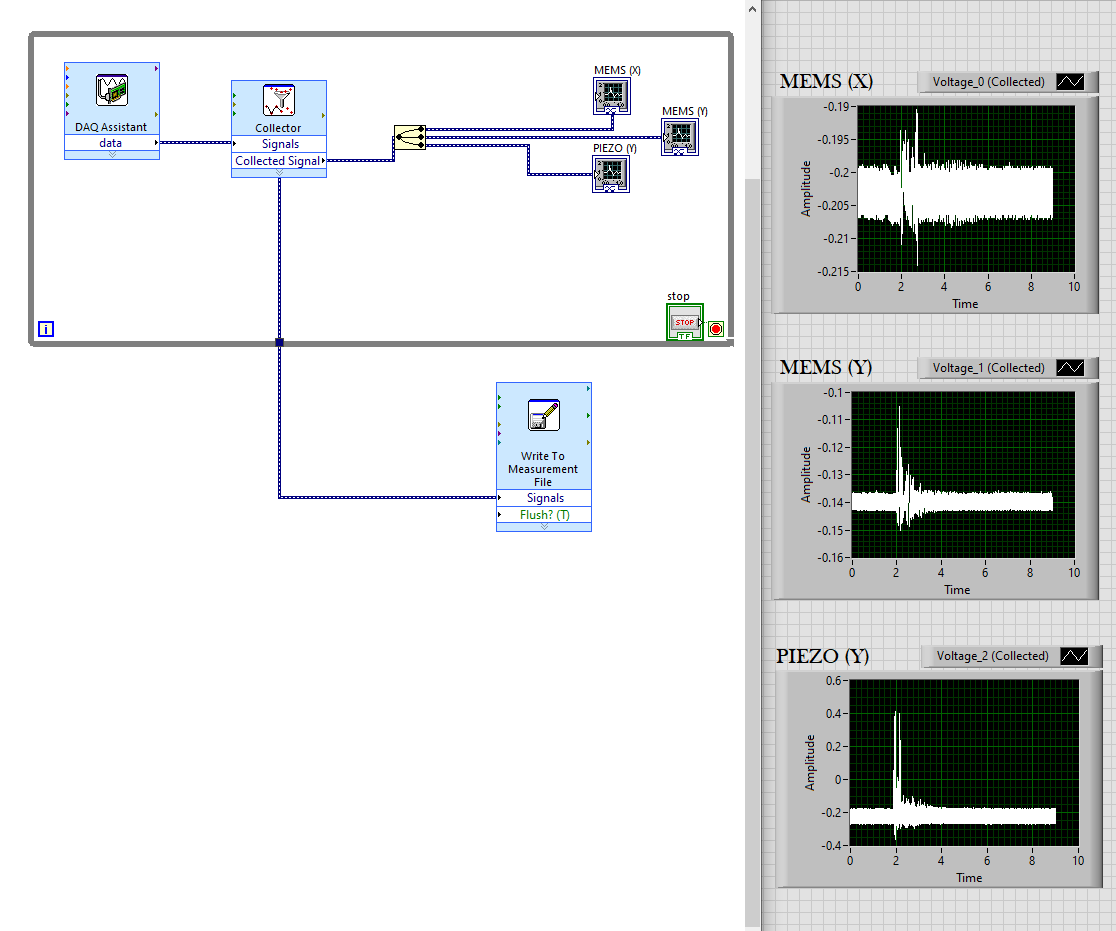
\includegraphics[width = 0.75\textwidth]{lab6images/blockdiagramlab6.PNG}
    \caption{LabVIEW Model Setup for Accelerometers}
    \label{fig:labview}
\end{figure}

\subsection{Accelerometer Setup and Experiment}
\begin{enumerate}
    \item  First, connect the MEMS and Piezoelectric accelerometers accordingly to power and ground, and connect the signal wires to corresponding NI-9215 ports. 
    \item Place the MEMS and Piezoelectric accelerometer on the wing model as shown in Figure \ref{fig:wingmodel}.
    \item Before hitting the wing with the brass mallet, the test that the MEMS and Piezoelectric accelerometers work by applying a force and observing the corresponding output in LabVIEW. Continue to the next step once working. If not working, check possible issues which may include:
    \begin{itemize}
        \item Connections on breadboard
        \item Faulty wires from NI-9215 Port
        \item Faulty accelerometer sensor
    \end{itemize}
    \item Run the LabVIEW model as shown in Figure \ref{fig:labview} and tap the wing with the brass mallet. Let it record the accelerometer data for 5 seconds. Save the data to a file and ensure it has been written correctly.
    \item Repeat previous step (3) for 10 measurements. 
    \item Once complete, we are ready to plot the measured accelerations and evaluate the data. From this we can identify the natural frequencies of the wing.
\end{enumerate}

\hypertarget{datapro}{}
\section{Data Processing}
\subsection{Variables and Equations}  

Newton's 2nd Law:

\begin{equation}
    a = \dfrac{F}{m}
\end{equation}

Variables:
\begin{enumerate}[label = \Roman*.]
    \item \( V \): Voltage
\end{enumerate}

    
\section{Results and Analysis}


\section{Conclusion}
In this lab experiment we learned how the piezoelectric and MEMS accelerometers operate in order to measure acceleration and perform frequency analysis of an aircraft surface. These devices are very practical in analyzing aircraft control surfaces that experience lots of vibration as these sensors are very responsive to forces. Analysis of these surfaces provides critical information useful to the structural dynamics of an aircraft. Due to this, accelerometers play an important role in ensuring an aircraft is safe to fly.

\newpage
\thispagestyle{empty}  % Clear header/footer
\begin{center}
	\vspace*{\fill}
	{\Huge Appendix}
	\vspace*{\fill}
\end{center}

% Start appendices
\newpage
\begin{appendices}
\pagestyle{fancy}
\renewcommand{\thefigure}{A\arabic{figure}}
\setcounter{figure}{0}

% \section*{t-Distribution Tables}
% \hypertarget{1}{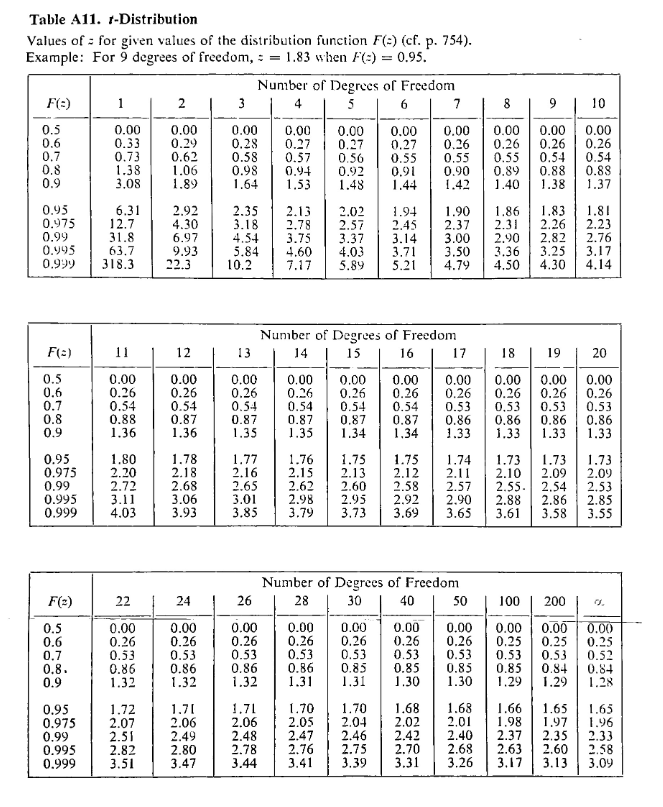
\includegraphics[width=0.95\textwidth]{t_distribution_Table_lecture3.png}}

\newpage

\section*{NI-9215 Datasheet}
\url{https://www.amc-systeme.de/files/pdf/ni-9215-amc.pdf}

\section*{IMI Series 660 Accelerometer Datasheet}
\url{https://pim-kft.hu/wp-content/uploads/2016/02/PCB_LowCost_Embeddable_Accelerometers.pdf}

\section*{ADXL335 Accelerometer Datasheet}
\url{https://www.analog.com/media/en/technical-documentation/data-sheets/adxl335.pdf}

\end{appendices}

\end{document}
